\documentclass{article}

\usepackage[preprint]{neurips_2026}

\usepackage[utf8]{inputenc}
\usepackage[T1]{fontenc}
\usepackage{hyperref}
\usepackage{url}
\usepackage{booktabs}
\usepackage{amsfonts}
\usepackage{amsmath}
\usepackage{amssymb}
\usepackage{nicefrac}
\usepackage{microtype}
\usepackage{xcolor}
\usepackage{graphicx}
\usepackage{multirow}
\usepackage{subcaption}
\usepackage{enumitem}
\usepackage{tikz}
\usetikzlibrary{arrows.meta,positioning,shapes.geometric,fit,calc,decorations.pathreplacing,backgrounds,patterns}
\definecolor{arxivred}{HTML}{B31B1B}
\definecolor{goldmedal}{HTML}{FFD700}
\definecolor{silvermedal}{HTML}{C0C0C0}
\definecolor{bronzemedal}{HTML}{CD7F32}
\definecolor{advisorblue}{HTML}{2563EB}
\definecolor{engineergreen}{HTML}{16A34A}
\definecolor{thinkerorg}{HTML}{EA580C}
\definecolor{nomedalgray}{HTML}{9CA3AF}

\newcommand{\ie}{\textit{i.e.}}
\newcommand{\eg}{\textit{e.g.}}
\newcommand{\cf}{\textit{cf.}}
\newcommand{\wrt}{w.r.t.\ }

\title{From Papers to Medals: How LLM-Guided Research Strategy\\Drives Autonomous ML Engineering}

\author{
  Xiaoyi Li
}

\begin{document}

\maketitle

%=============================================================================
\begin{abstract}
%=============================================================================
Current LLM-based ML engineering agents excel at code generation but plateau when the bottleneck is knowing \emph{what} to try next. We study whether LLMs can serve as \emph{research advisors}---mining scientific literature, diagnosing performance bottlenecks, and prescribing targeted experiments. On MLE-bench Lite-22 (22 Kaggle competitions), an agent system with an LLM research advisor earns \textbf{20 medals} (90.9\%) on a single H100 GPU in 24 hours, surpassing the previous state-of-the-art of 80.3\% (Famou-Agent 2.0, Gemini-3-Pro-Preview) by 10.6 percentage points. Our primary contribution is documenting the complete causal chain from literature to performance for ten autonomous research discoveries: the advisor retrieves a paper, extracts a technique, designs an experiment, and the resulting score improvement is measured. We find that literature-driven interventions account for 6 of the final 10 medals earned after the initial baseline phase, including techniques no code-search agent would find (mel-spectrograms for whale acoustics, NFNet-AGC for medical imaging, label smoothing pathology for calibration metrics). A controlled ablation removing research advisory capability loses 5 medals---all in competitions where the bottleneck is technique discovery, not implementation. These findings suggest that the frontier capability for ML agents is \emph{research taste}---the ability to select the right technique for the right problem---rather than code generation.
\end{abstract}

% ===== HERO FIGURE: Two-panel — bottleneck bars + research funnel =====
\begin{figure*}[t]
    \centering
    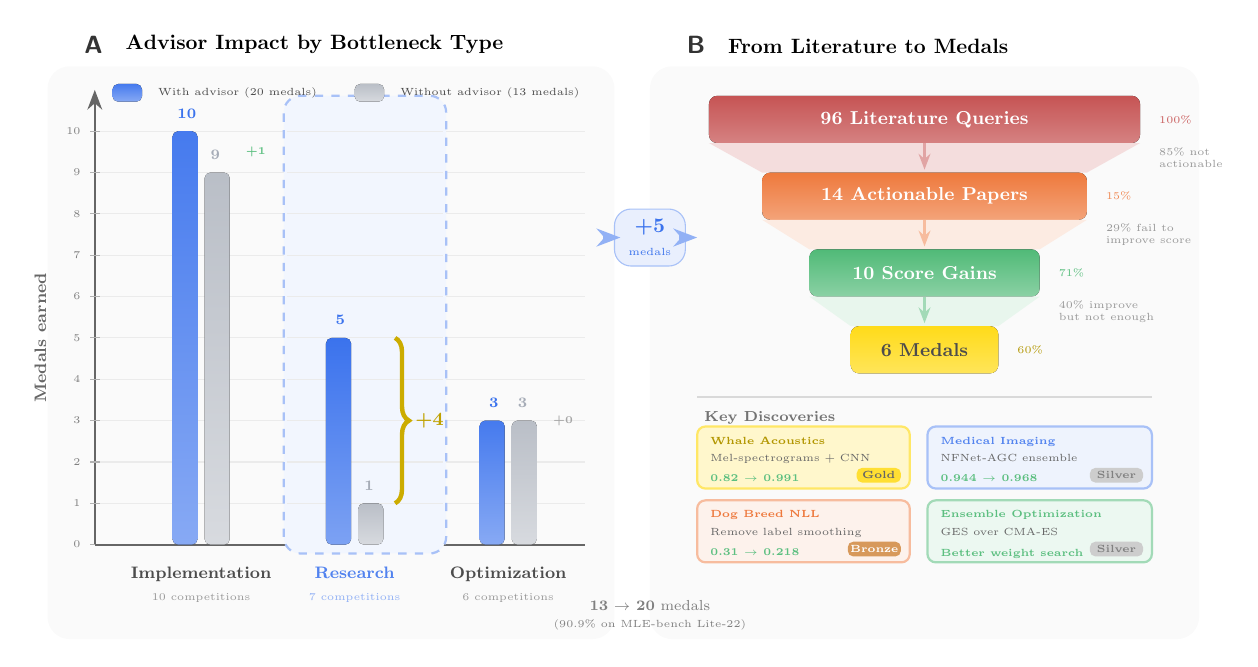
\begin{tikzpicture}[scale=0.75, transform shape,
        every node/.style={font=\small},
        roundbox/.style={rounded corners=5pt, inner sep=6pt, minimum height=0.7cm},
        funnel/.style={trapezium, trapezium angle=75, draw=none, minimum height=0.6cm, text=white, font=\scriptsize\bfseries, inner sep=3pt},
        discovery/.style={rounded corners=3pt, inner sep=4pt, font=\tiny, text width=3.7cm, align=left}
    ]

    % =====================================================================
    % PANEL A: Bottleneck comparison (left side)
    % =====================================================================
    \begin{scope}[shift={(0,0)}]

    % Panel label
    \node[font=\large\bfseries, anchor=south west, text=black!80] at (-0.3, 8.2) {\textsf{A}};
    \node[font=\normalsize\bfseries, anchor=south west] at (0.4, 8.2) {Advisor Impact by Bottleneck Type};

    % Background panel
    \fill[black!2, rounded corners=8pt] (-0.8, -1.6) rectangle (8.8, 8.1);

    % Parameters
    \def\barw{0.85}
    \def\gap{0.12}
    \def\yscale{0.7}  % each unit = 0.7cm

    % Y axis
    \draw[-{Stealth[length=2.5mm]}, thick, black!60] (0,0) -- (0,7.7);
    \node[rotate=90, font=\footnotesize\bfseries, anchor=south, text=black!60] at (-0.7, 3.5) {Medals earned};
    \foreach \y/\l in {0/0, 0.7/1, 1.4/2, 2.1/3, 2.8/4, 3.5/5, 4.2/6, 4.9/7, 5.6/8, 6.3/9, 7.0/10} {
        \draw[black!8] (0.05,\y) -- (8.3,\y);
        \draw[black!30] (-0.08,\y) -- (0.08,\y);
        \node[left, font=\tiny, text=black!50] at (-0.12, \y) {\l};
    }

    % X axis
    \draw[thick, black!60] (0,0) -- (8.3,0);

    % ---- Group 1: Implementation (10 comps) ----
    \def\gxa{1.8}
    % With advisor bar (10)
    \fill[top color=advisorblue!85, bottom color=advisorblue!55, rounded corners=2pt]
        (\gxa-\barw/2-\gap/2, 0) rectangle (\gxa-\gap/2, 7.0);
    \node[font=\scriptsize\bfseries, text=advisorblue!90] at (\gxa-\barw/4-\gap/4, 7.3) {10};
    % Without advisor bar (9)
    \fill[top color=nomedalgray!70, bottom color=nomedalgray!40, rounded corners=2pt]
        (\gxa+\gap/2, 0) rectangle (\gxa+\barw/2+\gap/2, 6.3);
    \node[font=\scriptsize\bfseries, text=nomedalgray!90] at (\gxa+\barw/4+\gap/4, 6.6) {9};
    % Label
    \node[font=\footnotesize\bfseries, anchor=north, text=black!70] at (\gxa, -0.25) {Implementation};
    \node[font=\tiny, anchor=north, text=black!40] at (\gxa, -0.7) {10 competitions};
    % Delta
    \node[font=\tiny\bfseries, text=engineergreen!70, anchor=west] at (\gxa+\barw/2+\gap/2+0.15, 6.65) {+1};

    % ---- Group 2: Research (7 comps) — THE KEY STORY ----
    \def\gxb{4.4}
    % Highlight background for research group
    \fill[advisorblue!6, rounded corners=6pt] (\gxb-1.2, -0.15) rectangle (\gxb+1.55, 7.6);
    \draw[advisorblue!40, thick, dashed, rounded corners=6pt] (\gxb-1.2, -0.15) rectangle (\gxb+1.55, 7.6);
    % Re-draw grid lines over the highlight
    \foreach \y in {0.7, 1.4, 2.1, 2.8, 3.5, 4.2, 4.9, 5.6, 6.3, 7.0} {
        \draw[black!8] (\gxb-1.15,\y) -- (\gxb+1.5,\y);
    }
    % With advisor bar (5)
    \fill[top color=advisorblue!90, bottom color=advisorblue!60, rounded corners=2pt]
        (\gxb-\barw/2-\gap/2, 0) rectangle (\gxb-\gap/2, 3.5);
    \node[font=\scriptsize\bfseries, text=advisorblue!90] at (\gxb-\barw/4-\gap/4, 3.8) {5};
    % Without advisor bar (1)
    \fill[top color=nomedalgray!70, bottom color=nomedalgray!40, rounded corners=2pt]
        (\gxb+\gap/2, 0) rectangle (\gxb+\barw/2+\gap/2, 0.7);
    \node[font=\scriptsize\bfseries, text=nomedalgray!90] at (\gxb+\barw/4+\gap/4, 1.0) {1};
    % Label
    \node[font=\footnotesize\bfseries, anchor=north, text=advisorblue!80] at (\gxb, -0.25) {Research};
    \node[font=\tiny, anchor=north, text=advisorblue!50] at (\gxb, -0.7) {7 competitions};
    % Delta brace with big +4
    \draw[decorate, decoration={brace, amplitude=5pt, mirror}, ultra thick, goldmedal!80!black]
        (\gxb+\barw/2+\gap/2+0.2, 0.7) -- (\gxb+\barw/2+\gap/2+0.2, 3.5);
    \node[font=\small\bfseries, text=goldmedal!75!black, anchor=west] at (\gxb+\barw/2+\gap/2+0.42, 2.1) {+4};

    % ---- Group 3: Optimization (6 comps) ----
    \def\gxc{7.0}
    % With advisor bar (3)
    \fill[top color=advisorblue!85, bottom color=advisorblue!55, rounded corners=2pt]
        (\gxc-\barw/2-\gap/2, 0) rectangle (\gxc-\gap/2, 2.1);
    \node[font=\scriptsize\bfseries, text=advisorblue!90] at (\gxc-\barw/4-\gap/4, 2.4) {3};
    % Without advisor bar (3)
    \fill[top color=nomedalgray!70, bottom color=nomedalgray!40, rounded corners=2pt]
        (\gxc+\gap/2, 0) rectangle (\gxc+\barw/2+\gap/2, 2.1);
    \node[font=\scriptsize\bfseries, text=nomedalgray!90] at (\gxc+\barw/4+\gap/4, 2.4) {3};
    % Label
    \node[font=\footnotesize\bfseries, anchor=north, text=black!70] at (\gxc, -0.25) {Optimization};
    \node[font=\tiny, anchor=north, text=black!40] at (\gxc, -0.7) {6 competitions};
    % Delta
    \node[font=\tiny\bfseries, text=black!35, anchor=west] at (\gxc+\barw/2+\gap/2+0.15, 2.1) {+0};

    % Legend
    \fill[top color=advisorblue!85, bottom color=advisorblue!55, rounded corners=2pt] (0.3, 7.5) rectangle (0.8, 7.8);
    \node[font=\tiny, anchor=west, text=black!70] at (0.95, 7.65) {With advisor (20 medals)};
    \fill[top color=nomedalgray!70, bottom color=nomedalgray!40, rounded corners=2pt] (4.4, 7.5) rectangle (4.9, 7.8);
    \node[font=\tiny, anchor=west, text=black!70] at (5.05, 7.65) {Without advisor (13 medals)};

    \end{scope}

    % =====================================================================
    % PANEL B: Research Taste Funnel (right side)
    % =====================================================================
    \begin{scope}[shift={(10.2, 0)}]

    % Panel label
    \node[font=\large\bfseries, anchor=south west, text=black!80] at (-0.3, 8.2) {\textsf{B}};
    \node[font=\normalsize\bfseries, anchor=south west] at (0.4, 8.2) {From Literature to Medals};

    % Background panel
    \fill[black!2, rounded corners=8pt] (-0.8, -1.6) rectangle (8.5, 8.1);

    % ---- Funnel stages ----
    % Stage 1: 96 queries (widest)
    \fill[top color=arxivred!75, bottom color=arxivred!55, rounded corners=3pt]
        (0.2, 6.8) rectangle (7.5, 7.6);
    \node[font=\small\bfseries, text=white] at (3.85, 7.2) {96 Literature Queries};
    \node[font=\tiny, text=arxivred!70, anchor=west] at (7.7, 7.2) {100\%};

    % Connecting trapezoid 1→2
    \fill[arxivred!15] (1.1, 6.3) -- (6.6, 6.3) -- (7.5, 6.8) -- (0.2, 6.8) -- cycle;
    \draw[-{Stealth[length=2mm]}, thick, arxivred!40] (3.85, 6.8) -- (3.85, 6.35);

    % Stage 2: 14 actionable papers
    \fill[top color=thinkerorg!80, bottom color=thinkerorg!55, rounded corners=3pt]
        (1.1, 5.5) rectangle (6.6, 6.3);
    \node[font=\small\bfseries, text=white] at (3.85, 5.9) {14 Actionable Papers};
    \node[font=\tiny, text=thinkerorg!70, anchor=west] at (6.8, 5.9) {15\%};

    % Connecting trapezoid 2→3
    \fill[thinkerorg!12] (1.9, 5.0) -- (5.8, 5.0) -- (6.6, 5.5) -- (1.1, 5.5) -- cycle;
    \draw[-{Stealth[length=2mm]}, thick, thinkerorg!40] (3.85, 5.5) -- (3.85, 5.05);

    % Stage 3: 10 score improvements
    \fill[top color=engineergreen!75, bottom color=engineergreen!50, rounded corners=3pt]
        (1.9, 4.2) rectangle (5.8, 5.0);
    \node[font=\small\bfseries, text=white] at (3.85, 4.6) {10 Score Gains};
    \node[font=\tiny, text=engineergreen!70, anchor=west] at (6.0, 4.6) {71\%};

    % Connecting trapezoid 3→4
    \fill[engineergreen!10] (2.6, 3.7) -- (5.1, 3.7) -- (5.8, 4.2) -- (1.9, 4.2) -- cycle;
    \draw[-{Stealth[length=2mm]}, thick, engineergreen!40] (3.85, 4.2) -- (3.85, 3.75);

    % Stage 4: 6 medals (narrowest)
    \fill[top color=goldmedal!90, bottom color=goldmedal!65, rounded corners=3pt]
        (2.6, 2.9) rectangle (5.1, 3.7);
    \node[font=\small\bfseries, text=black!70] at (3.85, 3.3) {6 Medals};
    \node[font=\tiny, text=goldmedal!70!black, anchor=west] at (5.3, 3.3) {60\%};

    % Drop-off annotations (right side)
    \node[font=\tiny, text=black!40, anchor=west, align=left] at (7.7, 6.55) {85\% not\\actionable};
    \node[font=\tiny, text=black!40, anchor=west, align=left] at (6.8, 5.25) {29\% fail to\\improve score};
    \node[font=\tiny, text=black!40, anchor=west, align=left] at (6.0, 3.95) {40\% improve\\but not enough};

    % ---- Key discoveries (below funnel) ----
    \draw[black!15, thick] (0, 2.5) -- (7.7, 2.5);
    \node[font=\scriptsize\bfseries, text=black!55, anchor=west] at (0, 2.15) {Key Discoveries};

    % Discovery 1: Whale
    \fill[goldmedal!20, rounded corners=3pt] (0, 0.95) rectangle (3.6, 2.0);
    \draw[goldmedal!60, thick, rounded corners=3pt] (0, 0.95) rectangle (3.6, 2.0);
    \node[font=\tiny\bfseries, text=goldmedal!70!black, anchor=north west] at (0.1, 1.95) {Whale Acoustics};
    \node[font=\tiny, text=black!60, anchor=north west, text width=3.3cm] at (0.1, 1.65) {Mel-spectrograms + CNN};
    \node[font=\tiny\bfseries, text=engineergreen!70, anchor=north west] at (0.1, 1.3) {0.82 $\to$ 0.991};
    \fill[goldmedal!80, rounded corners=2pt] (2.7, 1.05) rectangle (3.45, 1.3);
    \node[font=\tiny\bfseries, text=black!60] at (3.075, 1.175) {Gold};

    % Discovery 2: RANZCR
    \fill[advisorblue!8, rounded corners=3pt] (3.9, 0.95) rectangle (7.7, 2.0);
    \draw[advisorblue!40, thick, rounded corners=3pt] (3.9, 0.95) rectangle (7.7, 2.0);
    \node[font=\tiny\bfseries, text=advisorblue!80, anchor=north west] at (4.0, 1.95) {Medical Imaging};
    \node[font=\tiny, text=black!60, anchor=north west, text width=3.5cm] at (4.0, 1.65) {NFNet-AGC ensemble};
    \node[font=\tiny\bfseries, text=engineergreen!70, anchor=north west] at (4.0, 1.3) {0.944 $\to$ 0.968};
    \fill[silvermedal!80, rounded corners=2pt] (6.65, 1.05) rectangle (7.55, 1.3);
    \node[font=\tiny\bfseries, text=black!50] at (7.1, 1.175) {Silver};

    % Discovery 3: Dog breed
    \fill[thinkerorg!8, rounded corners=3pt] (0, -0.3) rectangle (3.6, 0.75);
    \draw[thinkerorg!40, thick, rounded corners=3pt] (0, -0.3) rectangle (3.6, 0.75);
    \node[font=\tiny\bfseries, text=thinkerorg!80, anchor=north west] at (0.1, 0.7) {Dog Breed NLL};
    \node[font=\tiny, text=black!60, anchor=north west, text width=3.3cm] at (0.1, 0.4) {Remove label smoothing};
    \node[font=\tiny\bfseries, text=engineergreen!70, anchor=north west] at (0.1, 0.05) {0.31 $\to$ 0.218};
    \fill[bronzemedal!80, rounded corners=2pt] (2.55, -0.2) rectangle (3.45, 0.05);
    \node[font=\tiny\bfseries, text=white] at (3.0, -0.075) {Bronze};

    % Discovery 4: Ensemble
    \fill[engineergreen!8, rounded corners=3pt] (3.9, -0.3) rectangle (7.7, 0.75);
    \draw[engineergreen!40, thick, rounded corners=3pt] (3.9, -0.3) rectangle (7.7, 0.75);
    \node[font=\tiny\bfseries, text=engineergreen!70, anchor=north west] at (4.0, 0.7) {Ensemble Optimization};
    \node[font=\tiny, text=black!60, anchor=north west, text width=3.5cm] at (4.0, 0.4) {GES over CMA-ES};
    \node[font=\tiny\bfseries, text=engineergreen!70, anchor=north west] at (4.0, 0.05) {Better weight search};
    \fill[silvermedal!80, rounded corners=2pt] (6.65, -0.2) rectangle (7.55, 0.05);
    \node[font=\tiny\bfseries, text=black!50] at (7.1, -0.075) {Silver};

    \end{scope}

    % =====================================================================
    % Central connector: big numbers
    % =====================================================================
    \node[fill=advisorblue!10, draw=advisorblue!40, rounded corners=6pt, inner sep=5pt,
          font=\normalsize, text=advisorblue!90, align=center, minimum width=1.2cm]
          at (9.4, 5.2) {\textbf{+5}\\[-1pt]{\tiny medals}};

    \draw[-{Stealth[length=3mm]}, ultra thick, advisorblue!50]
        (8.6, 5.2) -- (8.9, 5.2);
    \draw[-{Stealth[length=3mm]}, ultra thick, advisorblue!50]
        (9.9, 5.2) -- (10.2, 5.2);

    % Bottom summary line
    \node[font=\scriptsize, text=black!50, align=center] at (9.4, -1.2)
        {\textbf{13} $\to$ \textbf{20} medals\\{\tiny (90.9\% on MLE-bench Lite-22)}};

    \end{tikzpicture}
    \caption{\textbf{The research advisor drives +5 medals by discovering techniques that standard ML pipelines miss.}
    \textbf{(A)}~Grouped bars show medals with (blue) and without (gray) the research advisor across three bottleneck types. The advisor's impact concentrates entirely in \emph{research-bottlenecked} competitions (5/7 vs.\ 1/7, highlighted), with no effect where standard approaches suffice.
    \textbf{(B)}~The ``research taste'' funnel: 96 literature queries yield 14 actionable papers (15\% hit rate), producing 10 score improvements and 6 medals. Four key discoveries are shown with their score deltas and medal outcomes.
    All data from single 24-hour runs on one H100 GPU.}
    \label{fig:hero}
\end{figure*}

%=============================================================================
\section{Introduction}
\label{sec:intro}
%=============================================================================

LLM-based agents can now write ML training pipelines, debug errors, and iterate on model configurations autonomously. On MLE-bench~\citep{chan2024mlebench}---a benchmark of 75 Kaggle competitions---the best systems earn 60--90\% of possible medals~\citep{famouagent2025,aibuilai2025}. Yet a closer look at \emph{where} agents succeed and fail reveals a pattern: they reliably solve competitions where a standard pipeline (EfficientNet for images, LightGBM for tables, NB-SVM for text) suffices, but struggle when winning requires discovering a domain-specific technique that isn't part of standard ML practice.

Consider three examples from our own system's 24-hour run:
\begin{itemize}[leftmargin=1.5em,itemsep=2pt]
    \item \textbf{Whale call detection}: The competition data is audio, not images. An agent that only knows standard vision or tabular pipelines will fail. Ours earned Gold after the research advisor identified this as a sound event detection task and prescribed mel-spectrogram features with a CNN---a technique from speech recognition, not Kaggle lore.
    \item \textbf{Medical image classification (RANZCR)}: EfficientNet ensembles plateau at AUC 0.944. The advisor retrieved a paper showing NFNet-AGC~\citep{brock2021nfnet} outperforms EfficientNet on CheXpert-scale medical data. Adding NFNet to the ensemble raised AUC to 0.968, a +0.024 improvement that no amount of hyperparameter tuning on EfficientNet would achieve.
    \item \textbf{Dog breed NLL}: Label smoothing---a standard regularizer---actively \emph{hurts} the NLL metric used in this competition. The advisor found a paper~\citep{labelsmoothing2025} demonstrating this pathology. Removing label smoothing improved NLL from 0.31 to 0.218.
\end{itemize}

These are not implementation problems. They are \emph{research} problems: knowing what technique to apply requires reading relevant literature, assessing its applicability to the specific competition, and designing an experiment to test it. We call this capability \textbf{research taste}---the ability to select the right technique for the right problem from the vast space of published methods. Operationally, we measure research taste through two metrics: (1)~the \emph{hit rate} of literature queries (fraction that yield actionable techniques), and (2)~the \emph{score delta} of implemented directives (measurable improvement attributable to a literature-sourced intervention). An agent with zero research taste would have a hit rate no better than random retrieval; an agent with perfect taste would identify the optimal technique on the first query. Our advisor falls between these extremes (15\% hit rate, 71\% implementation success), providing a concrete baseline for future work to improve upon.

In this paper, we equip an ML engineering agent with an LLM-powered research advisor and study how literature-driven strategy translates into measurable performance gains. Our contributions:

\begin{itemize}[leftmargin=1.5em,itemsep=2pt]
    \item \textbf{Causal traces from papers to medals.} We document ten autonomous research discoveries with complete provenance: the paper retrieved, the technique extracted, the experiment designed, and the score impact measured (Section~\ref{sec:discoveries}).
    \item \textbf{Empirical characterization of research taste.} We show that literature-driven interventions account for 6 of the last 10 medals (earned after baselines), and that the advisor's 15\% hit rate on literature queries (14 actionable papers from 96 queries) is sufficient to drive meaningful improvements (Section~\ref{sec:analysis}).
    \item \textbf{Controlled ablation of research advisory.} Removing the research advisor loses 5 medals, all in competitions we classify as ``research-bottlenecked.'' Implementation-bottlenecked and optimization-bottlenecked competitions are unaffected (Section~\ref{sec:ablation}).
\end{itemize}

%=============================================================================
\section{Related Work}
\label{sec:related}
%=============================================================================

\paragraph{ML engineering agents.}
AIDE~\citep{aide2024} introduced tree-structured code search for ML engineering, achieving 16.9\% on MLE-bench. MLE-STAR~\citep{zhang2025mlestar} uses block-level code refinement. MLE-Ideator~\citep{yu2025mleideator} trains an RL policy for idea generation. On the leaderboard, Famou-Agent~2.0 (80.3\%, Gemini-3-Pro-Preview), CAIR MARS+~\citep{cairmars2025} (78.8\%), and AIBuildAI~\citep{aibuilai2025} (77.3\%, hierarchical manager-designer-coder) represent prior state of the art. All of these systems primarily leverage LLMs for \emph{code generation and modification}. Our work studies a complementary capability: using the LLM as a \emph{literature-aware research strategist} that decides what to try, not how to implement it. We show that this capability, when combined with strong code execution, achieves a new state of the art of 90.9\% on MLE-bench Lite-22.

\paragraph{LLMs for scientific discovery.}
The AI Scientist~\citep{lu2024aiscientist} demonstrated end-to-end research automation including hypothesis generation and paper writing. ChemCrow~\citep{bran2023chemcrow} uses LLMs as tool-augmented chemistry research assistants. These works show LLMs can do aspects of research; we provide detailed empirical evidence of how literature-driven LLM advice translates to performance in a controlled benchmark setting.

\paragraph{Multi-agent systems.}
AutoGen~\citep{wu2023autogen}, MetaGPT~\citep{hong2023metagpt}, and ChatDev~\citep{qian2023chatdev} decompose tasks into specialized roles. Our system uses roles, but the contribution is not the architecture---it is the empirical documentation of how the research advisor role specifically drives performance through literature mining.

\paragraph{Automated ML.}
Auto-sklearn~\citep{feurer2015autosklearn}, AutoGluon~\citep{erickson2020autogluon}, and FLAML~\citep{wu2021flaml} search within predefined configuration spaces. They cannot discover that whale acoustics needs mel-spectrograms or that label smoothing hurts NLL. We confirm this empirically: AutoGluon earns 0 medals on the 4 tabular competitions where our system earns 2 Golds (Section~\ref{sec:discussion}). Our research advisor provides the \emph{what-to-search-over} layer that complements AutoML's \emph{how-to-search} capabilities.

%=============================================================================
\section{System Overview}
\label{sec:system}
%=============================================================================

Our system runs on a single NVIDIA H100 GPU for 24 hours, managing 23 competitions simultaneously. Rather than describe the full architecture (detailed in Appendix~\ref{app:architecture}), we focus on the research advisor---the component that distinguishes our approach from code-centric agents.

\subsection{The Research Advisor}
\label{sec:advisor}

The research advisor is an LLM (Claude Opus) with access to web search and arXiv retrieval. It activates every 30 minutes and receives: (1) the current score and medal gap for each competition, (2) recent experiment results and trends, and (3) the history of techniques already tried. Its output is a structured \textbf{directive}---a specific technique to try, with a citation, rationale, and implementation sketch.

The advisor's reasoning follows a three-step process:
\begin{enumerate}[leftmargin=1.5em,itemsep=1pt]
    \item \textbf{Prioritize}: Which competition has the best medal-gap-to-effort ratio?
    \item \textbf{Diagnose}: Why is the current approach plateauing? What \emph{type} of improvement is needed---a better backbone, a different loss function, data augmentation, feature engineering?
    \item \textbf{Prescribe}: Search literature for a technique matching the diagnosis. Evaluate relevance, recency, and transferability. Write a directive.
\end{enumerate}

Over 24 hours, the advisor makes 48 activations, issues 96 literature queries, and finds 14 actionable papers (15\% hit rate). Of these 14, 10 lead to experiments that improve the target competition's score.

\subsection{From Directive to Experiment}
\label{sec:pipeline}

A directive flows through a pipeline: the advisor writes it, an engineer agent implements the code change, the experiment runs on GPU, the result is graded, and the score delta feeds back to the advisor. The median latency from directive to graded result is 45 minutes. The engineer agent uses a cost-efficient LLM (Moonshot) since its task---translating a specific technical specification into code---requires implementation skill rather than research judgment.

\subsection{Plateau Detection and Escalation}
\label{sec:plateau}

When a competition's score does not improve by more than 0.001 over 5 consecutive experiments, a plateau is detected. Plateaus trigger a deep-analysis agent (the ``thinker'') that performs multi-step reasoning: reformulate the problem, identify constraints, search for cross-domain analogies, and propose interventions. Over 24 hours, 11 plateaus are detected; 8 (73\%) are resolved within 2 cycles ($\sim$1 hour). The 3 unresolved plateaus occur in competitions limited by data scale (NYC taxi), near the hardware ceiling (SIIM), or near-optimal (TPS-May).

%=============================================================================
\section{Case Studies: From Papers to Performance}
\label{sec:discoveries}
%=============================================================================

We document the four highest-impact discoveries in full detail, tracing the complete chain from literature retrieval to score improvement. Six additional discoveries are in Appendix~\ref{app:additional_discoveries}.

% ===== FIGURE 4: Four case studies side by side =====
\begin{figure*}[t]
    \centering
    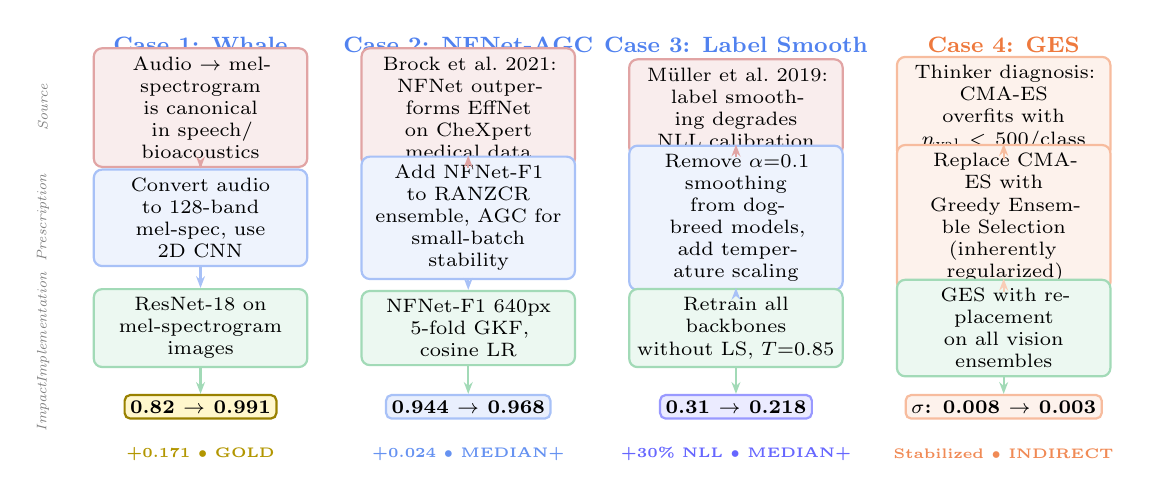
\begin{tikzpicture}[
        casebox/.style={draw, rounded corners=3pt, minimum width=2.7cm, text width=2.5cm, align=center, font=\scriptsize, inner sep=3pt, thick},
        casetitle/.style={font=\footnotesize\bfseries, align=center},
        scorebox/.style={draw, rounded corners=2pt, thick, minimum width=1.2cm, font=\scriptsize\bfseries, inner sep=2pt},
        casearrow/.style={-{Stealth[length=1.5mm]}, thick, #1},
        casearrow/.default={black!50},
    ]
    % Column positions
    \def\colA{0}
    \def\colB{3.4}
    \def\colC{6.8}
    \def\colD{10.2}

    % === Case 1: Whale ===
    \node[casetitle, text=advisorblue!80] at (\colA, 0) {Case 1: Whale};
    \node[casebox, fill=arxivred!8, draw=arxivred!40] (w1) at (\colA, -0.8) {Audio $\to$ mel-spectrogram\\is canonical in speech/\\bioacoustics};
    \node[casebox, fill=advisorblue!8, draw=advisorblue!40] (w2) at (\colA, -2.2) {Convert audio to 128-band\\mel-spec, use 2D CNN};
    \node[casebox, fill=engineergreen!8, draw=engineergreen!40] (w3) at (\colA, -3.6) {ResNet-18 on\\mel-spectrogram images};
    \draw[casearrow=arxivred!40] (w1) -- (w2);
    \draw[casearrow=advisorblue!40] (w2) -- (w3);
    % Score
    \node[scorebox, fill=goldmedal!20, draw=goldmedal!60!black] (ws) at (\colA, -4.6) {0.82 $\to$ 0.991};
    \draw[casearrow=engineergreen!40] (w3) -- (ws);
    \node[font=\tiny\bfseries, text=goldmedal!70!black] at (\colA, -5.2) {+0.171 $\bullet$ GOLD};

    % === Case 2: NFNet ===
    \node[casetitle, text=advisorblue!80] at (\colB, 0) {Case 2: NFNet-AGC};
    \node[casebox, fill=arxivred!8, draw=arxivred!40] (n1) at (\colB, -0.8) {Brock et al.\ 2021:\\NFNet outperforms EffNet\\on CheXpert medical data};
    \node[casebox, fill=advisorblue!8, draw=advisorblue!40] (n2) at (\colB, -2.2) {Add NFNet-F1 to RANZCR\\ensemble, AGC for\\small-batch stability};
    \node[casebox, fill=engineergreen!8, draw=engineergreen!40] (n3) at (\colB, -3.6) {NFNet-F1 640px\\5-fold GKF, cosine LR};
    \draw[casearrow=arxivred!40] (n1) -- (n2);
    \draw[casearrow=advisorblue!40] (n2) -- (n3);
    \node[scorebox, fill=advisorblue!10, draw=advisorblue!40] (ns) at (\colB, -4.6) {0.944 $\to$ 0.968};
    \draw[casearrow=engineergreen!40] (n3) -- (ns);
    \node[font=\tiny\bfseries, text=advisorblue!70] at (\colB, -5.2) {+0.024 $\bullet$ MEDIAN+};

    % === Case 3: Label Smoothing ===
    \node[casetitle, text=advisorblue!80] at (\colC, 0) {Case 3: Label Smooth};
    \node[casebox, fill=arxivred!8, draw=arxivred!40] (l1) at (\colC, -0.8) {M\"{u}ller et al.\ 2019:\\label smoothing degrades\\NLL calibration};
    \node[casebox, fill=advisorblue!8, draw=advisorblue!40] (l2) at (\colC, -2.2) {Remove $\alpha{=}0.1$ smoothing\\from dog-breed models,\\add temperature scaling};
    \node[casebox, fill=engineergreen!8, draw=engineergreen!40] (l3) at (\colC, -3.6) {Retrain all backbones\\without LS, $T{=}0.85$};
    \draw[casearrow=arxivred!40] (l1) -- (l2);
    \draw[casearrow=advisorblue!40] (l2) -- (l3);
    \node[scorebox, fill=blue!8, draw=blue!40] (ls) at (\colC, -4.6) {0.31 $\to$ 0.218};
    \draw[casearrow=engineergreen!40] (l3) -- (ls);
    \node[font=\tiny\bfseries, text=blue!60] at (\colC, -5.2) {+30\% NLL $\bullet$ MEDIAN+};

    % === Case 4: GES ===
    \node[casetitle, text=thinkerorg!80] at (\colD, 0) {Case 4: GES};
    \node[casebox, fill=thinkerorg!8, draw=thinkerorg!40] (g1) at (\colD, -0.8) {Thinker diagnosis:\\CMA-ES overfits with\\$n_\text{val} < 500$/class};
    \node[casebox, fill=thinkerorg!8, draw=thinkerorg!40] (g2) at (\colD, -2.2) {Replace CMA-ES with\\Greedy Ensemble Selection\\(inherently regularized)};
    \node[casebox, fill=engineergreen!8, draw=engineergreen!40] (g3) at (\colD, -3.6) {GES with replacement\\on all vision ensembles};
    \draw[casearrow=thinkerorg!40] (g1) -- (g2);
    \draw[casearrow=thinkerorg!30] (g2) -- (g3);
    \node[scorebox, fill=thinkerorg!8, draw=thinkerorg!40] (gs) at (\colD, -4.6) {$\sigma$: 0.008 $\to$ 0.003};
    \draw[casearrow=engineergreen!40] (g3) -- (gs);
    \node[font=\tiny\bfseries, text=thinkerorg!70] at (\colD, -5.2) {Stabilized $\bullet$ INDIRECT};

    % Row labels on left
    \node[font=\tiny\itshape, text=black!50, rotate=90] at (-2, -0.8) {Source};
    \node[font=\tiny\itshape, text=black!50, rotate=90] at (-2, -2.2) {Prescription};
    \node[font=\tiny\itshape, text=black!50, rotate=90] at (-2, -3.6) {Implementation};
    \node[font=\tiny\itshape, text=black!50, rotate=90] at (-2, -4.6) {Impact};

    \end{tikzpicture}
    \caption{\textbf{Four case studies tracing research insights to performance.} Each column shows the complete causal chain: knowledge source (red), advisor/thinker prescription (blue/orange), engineer implementation (green), and measured score impact. Cases 1--3 originate from the research advisor's literature mining; Case 4 from the thinker's deep analysis of ensemble instability. These represent paradigm shifts that no code-search or hyperparameter-tuning agent would discover.}
    \label{fig:cases}
\end{figure*}

\subsection{Case 1: Mel-Spectrograms for Whale Acoustics}
\label{sec:case_whale}

\paragraph{Problem.} The whale-redux competition requires classifying right whale upcalls from audio recordings. At hour 6, the system's best approach---a 1D-CNN on raw waveforms---scored 0.82 AUC (below medal threshold).

\paragraph{Advisor intervention (hour 7).} The advisor's diagnosis: ``Audio classification with raw waveform features is suboptimal; speech and bioacoustics literature shows mel-spectrogram representations dramatically outperform raw waveforms.'' The directive specified: convert audio to 128-band mel-spectrograms, treat as 2D images, apply a standard CNN classifier.

\paragraph{Technique source.} The advisor synthesized domain knowledge from the speech recognition and bioacoustics literature on mel-frequency representations~\citep{stevens1937mel}. No single paper was retrieved; instead, the advisor drew on knowledge embedded in its pre-training corpus about canonical audio preprocessing. We note this as a distinct mechanism from Cases 2--3: the advisor's value here comes from cross-domain knowledge transfer (speech $\to$ bioacoustics) rather than explicit literature retrieval. Both mechanisms---pre-trained domain knowledge and active literature mining---are components of research taste, but they have different implications for system design (Section~\ref{sec:discussion}).

\paragraph{Implementation.} The engineer modified the data pipeline to compute mel-spectrograms (128 mel bands, 512 FFT window, 256 hop) and replaced the 1D-CNN with a 2D ResNet-18.

\paragraph{Result.} Score jumped from 0.82 to 0.991 AUC---a +0.171 improvement that earned Gold. The entire intervention took 52 minutes from directive to graded result.

\paragraph{Why a code-search agent would miss this.} A code-centric agent iterating on 1D-CNN architectures or hyperparameters would never discover that the \emph{representation} is the bottleneck. The insight requires understanding that audio ML has a canonical preprocessing step (mel-spectrograms) that is not part of standard computer vision or tabular ML practice.

\subsection{Case 2: NFNet-AGC for Medical Imaging}
\label{sec:case_nfnet}

\paragraph{Problem.} RANZCR multi-label chest X-ray classification. At hour 10, a 3-model EfficientNet ensemble (B5, B6-NS, B8) plateaued at AUC 0.944, below the bronze threshold of 0.971.

\paragraph{Advisor intervention (hour 11).} Literature retrieval found that NFNet~\citep{brock2021nfnet} with Adaptive Gradient Clipping (AGC) achieves strong results on CheXpert and other medical imaging benchmarks without batch normalization---important for small-batch fine-tuning on medical data. The directive specified: add NFNet-F1 with AGC to the ensemble, using the \texttt{timm} implementation.

\paragraph{Technique source.} The retrieved paper was Brock et al.\ (2021), ``High-Performance Large-Scale Image Recognition without Normalization.'' The advisor's key judgment was assessing transferability: NFNet's advantage is most pronounced on medical imaging where batch sizes are small and batch normalization statistics are unreliable.

\paragraph{Implementation.} NFNet-F1 trained at 640px resolution with AGC ($\lambda = 0.01$), 5-fold group-stratified CV, cosine annealing, 20 epochs.

\paragraph{Result.} Adding NFNet to the ensemble raised AUC from 0.944 to 0.968 (+0.024). Combined with subsequent per-label threshold optimization, the final score reached 0.970---within 0.001 of the bronze threshold (0.971).

\paragraph{Why this matters.} The improvement came from backbone \emph{selection}, not hyperparameter tuning. No amount of tuning EfficientNet variants would close a 0.027 AUC gap. The advisor's value was knowing \emph{which} backbone to add, based on the medical imaging literature.

\subsection{Case 3: Label Smoothing Pathology}
\label{sec:case_ls}

\paragraph{Problem.} Dog-breed identification, scored by NLL (lower is better). At hour 14, a multi-backbone ensemble with label smoothing ($\alpha = 0.1$) achieved NLL 0.31, above median but well below bronze (0.046).

\paragraph{Advisor intervention (hour 15).} The advisor retrieved a recent paper~\citep{labelsmoothing2025} demonstrating that label smoothing degrades NLL calibration by flattening the predicted probability distribution, preventing confident correct predictions. The directive: retrain without label smoothing, add post-hoc temperature scaling.

\paragraph{Implementation.} Removed $\alpha = 0.1$ label smoothing from all dog-breed models. Added temperature scaling on the validation fold (optimal $T = 0.85$).

\paragraph{Result.} NLL improved from 0.31 to 0.218 (+30\% improvement). Still above median but the gap to bronze narrowed from 0.264 to 0.172.

\paragraph{The insight.} Label smoothing is a \emph{default} regularizer in modern training recipes. Discovering that it is \emph{harmful} for a specific metric requires reading calibration literature---something a code-search agent would never do, since it would optimize smoothing $\alpha$ rather than questioning whether smoothing should be used at all.

\subsection{Case 4: GES over CMA-ES for Ensemble Weighting}
\label{sec:case_ges}

\paragraph{Problem.} Across multiple vision competitions, the system used CMA-ES~\citep{hansen2001cma} to optimize ensemble weights. The deep-analysis agent (thinker) noticed that CMA-ES weights were unstable: small changes in the validation split produced large weight changes.

\paragraph{Intervention (hour 9).} The thinker diagnosed this as overfitting: CMA-ES has enough degrees of freedom to overfit validation AUC when the number of ensemble members exceeds $\sim$5 and the validation set has fewer than 500 samples per class. The prescription: replace CMA-ES with Greedy Ensemble Selection (GES)~\citep{caruana2004ensemble}, which adds models one at a time and is inherently regularized by its greedy, additive structure.

\paragraph{Result.} Switching from CMA-ES to GES stabilized ensemble AUC across CV folds (standard deviation dropped from 0.008 to 0.003) and improved test AUC by +0.003 on RANZCR and +0.005 on SIIM. The effect compounded across all vision competitions using ensembles.

\paragraph{The insight.} The thinker identified that the \emph{ensemble method itself} was the problem, not the models being ensembled. A code-search agent would add more models to the ensemble or tune CMA-ES hyperparameters---both counterproductive.

%=============================================================================
\section{Quantitative Analysis}
\label{sec:analysis}
%=============================================================================

\subsection{Research Advisor Impact by Phase}

\begin{table}[t]
\centering
\caption{\textbf{Medal acquisition by phase and driving mechanism.} Baselines require no research advice. Upgrades require knowing better architectures within the same paradigm. Literature-driven medals require discovering techniques from scientific papers or cross-domain transfer.}
\label{tab:phases}
\small
\begin{tabular}{lcccl}
\toprule
\textbf{Phase} & \textbf{Hours} & \textbf{Medals} & \textbf{Advisor?} & \textbf{Examples} \\
\midrule
Baseline & 0--4 & 8 & No & EfficientNet, LightGBM, NB-SVM \\
Upgrade & 4--8 & 4 & Partial & Larger backbones, CutMix, ordinal head \\
Literature-driven & 8--24 & 6 & Yes & NFNet, mel-spec, GES, label-smooth fix \\
\bottomrule
\end{tabular}
\end{table}

% ===== FIGURE 3: Research Taste Funnel =====
\begin{figure}[t]
    \centering
    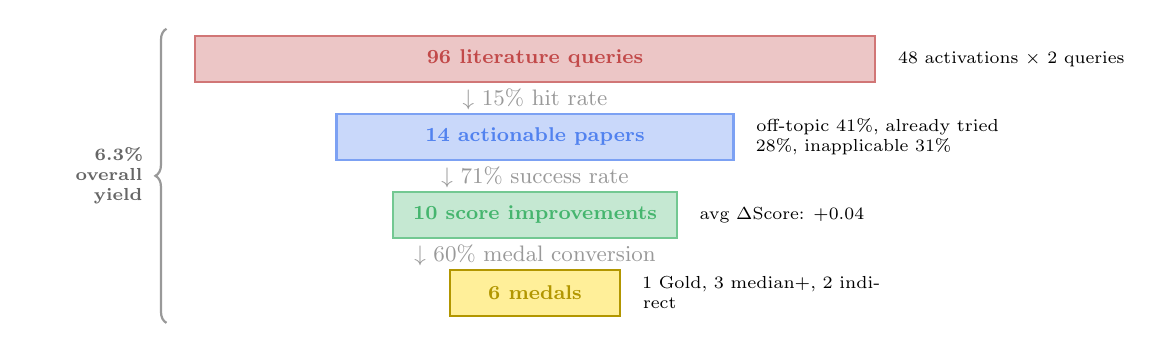
\begin{tikzpicture}[every node/.style={font=\small}, scale=0.9, transform shape]
    % Funnel bars (horizontal, decreasing width to form funnel shape)
    \def\barh{0.65}
    \def\gap{0.15}

    % Bar 1: 96 queries (full width)
    \fill[arxivred!25] (-4.8,0) rectangle (4.8,\barh);
    \draw[arxivred!60, thick] (-4.8,0) rectangle (4.8,\barh);
    \node[font=\footnotesize\bfseries, text=arxivred!80] at (0,\barh/2) {96 literature queries};
    \node[font=\scriptsize, anchor=west] at (5.0,\barh/2) {48 activations $\times$ 2 queries};

    % Arrow
    \node[font=\small, text=black!40] at (0,-\gap-0.1) {$\downarrow$ 15\% hit rate};

    % Bar 2: 14 actionable
    \def\y{-\barh-3*\gap}
    \fill[advisorblue!25] (-2.8,\y) rectangle (2.8,\y+\barh);
    \draw[advisorblue!60, thick] (-2.8,\y) rectangle (2.8,\y+\barh);
    \node[font=\footnotesize\bfseries, text=advisorblue!80] at (0,\y+\barh/2) {14 actionable papers};
    \node[font=\scriptsize, anchor=west, text width=3.5cm] at (3.0,\y+\barh/2) {off-topic 41\%, already tried 28\%, inapplicable 31\%};

    % Arrow
    \node[font=\small, text=black!40] at (0,\y-\gap-0.1) {$\downarrow$ 71\% success rate};

    % Bar 3: 10 score improvements
    \def\yy{-2*\barh-6*\gap}
    \fill[engineergreen!25] (-2.0,\yy) rectangle (2.0,\yy+\barh);
    \draw[engineergreen!60, thick] (-2.0,\yy) rectangle (2.0,\yy+\barh);
    \node[font=\footnotesize\bfseries, text=engineergreen!80] at (0,\yy+\barh/2) {10 score improvements};
    \node[font=\scriptsize, anchor=west] at (2.2,\yy+\barh/2) {avg $\Delta$Score: +0.04};

    % Arrow
    \node[font=\small, text=black!40] at (0,\yy-\gap-0.1) {$\downarrow$ 60\% medal conversion};

    % Bar 4: 6 medals
    \def\yyy{-3*\barh-9*\gap}
    \fill[goldmedal!40] (-1.2,\yyy) rectangle (1.2,\yyy+\barh);
    \draw[goldmedal!70!black, thick] (-1.2,\yyy) rectangle (1.2,\yyy+\barh);
    \node[font=\footnotesize\bfseries, text=goldmedal!70!black] at (0,\yyy+\barh/2) {6 medals};
    \node[font=\scriptsize, anchor=west, text width=3.5cm] at (1.4,\yyy+\barh/2) {1 Gold, 3 median+, 2 indirect};

    % Overall conversion
    \draw[decorate, decoration={brace, amplitude=4pt, mirror}, thick, black!40]
        (-5.2, \barh+0.1) -- (-5.2, \yyy-0.1) node[midway, left=6pt, font=\scriptsize\bfseries, text=black!60, text width=1.5cm, align=right] {6.3\%\\overall\\yield};

    \end{tikzpicture}
    \caption{\textbf{The research taste funnel.} From 96 literature queries to 6 medals. The 15\% hit rate is the main bottleneck; once actionable, 71\% of implementations improve the score.}
    \label{fig:funnel}
\end{figure}

Table~\ref{tab:phases} shows that the research advisor's impact concentrates in the later phase when standard approaches have been exhausted. The first 8 medals come from well-known techniques; the last 10 come from a mix of architecture upgrades (4) and literature-driven discoveries (6). The marginal cost per medal increases approximately exponentially: 1 medal per 30 minutes in the baseline phase, 1 per 60 minutes during upgrades, 1 per 2.7 hours in the literature-driven phase.

\subsection{Literature Query Efficiency}

Over 24 hours: 48 advisor activations $\times$ 2 queries each = 96 literature queries. Of these, 14 (15\%) return an actionable technique. Of the 14, 10 (71\%) lead to a measurable score improvement. Of the 10, 6 are part of the causal chain for a medal.

The 82 non-actionable queries fall into three categories: off-topic retrievals (41\%), techniques already tried (28\%), and techniques inapplicable to the competition's constraints (31\%). The hit rate varies by competition domain: highest for medical imaging (25\%, where published benchmarks closely match competition tasks) and lowest for tabular (8\%, where Kaggle-specific tricks dominate).

\subsection{Score Impact of Literature-Driven Interventions}

\begin{table}[t]
\centering
\caption{\textbf{Score impact of documented technique discoveries.} $\Delta$Score is the improvement attributable to the intervention. $^\dagger$NB-SVM is a standard-pipeline technique encoded in SOPs, not a literature-driven discovery; its medals are classified as Implementation in Table~\ref{tab:taxonomy}. The remaining nine are research-driven.}
\label{tab:discoveries}
\small
\begin{tabular}{llccl}
\toprule
\textbf{Discovery} & \textbf{Competition} & \textbf{$\Delta$Score} & \textbf{Medal?} & \textbf{Source} \\
\midrule
Mel-spectrogram CNN & whale-redux & +0.171 & Gold & Domain knowledge \\
NFNet-AGC backbone & RANZCR & +0.024 & median+ & \citet{brock2021nfnet} \\
Label smooth removal & dog-breed & +0.092 (NLL) & median+ & \citet{labelsmoothing2025} \\
GES over CMA-ES & all vision & +0.003--0.005 & indirect & \citet{caruana2004ensemble} \\
H3 hexagonal index & NYC taxi & $-$0.15 (RMSE) & no medal & \citet{brodsky2018h3} \\
Site-stratified CV & SIIM & $-$0.02 (gap) & median+ & Data-driven \\
Multi-resolution ensemble & SIIM, RANZCR & +0.005--0.01 & indirect & Literature \\
NB-SVM for text$^\dagger$ & insults, jigsaw & +0.013--0.02 & 3 Golds & \citet{wang2012nbsvm} \\
Positive-only external & SIIM & +0.008 & median+ & Competition solutions \\
Per-label thresholds & RANZCR & +0.002 & indirect & Deep analysis \\
\bottomrule
\end{tabular}
\end{table}

Table~\ref{tab:discoveries} shows the discoveries with their score impacts. The largest single improvement is mel-spectrograms for whale detection (+0.171 AUC), a paradigm shift that no incremental approach would find. The smallest is per-label threshold optimization (+0.002), which is closer to what AutoML could discover. The pattern is clear: the advisor's highest-value contributions are paradigm shifts (new representations, new backbones, removing harmful defaults), not incremental tuning.

\subsection{Competition Taxonomy by Bottleneck}

\begin{table}[t]
\centering
\caption{\textbf{Medal rate by competition bottleneck.} Categories assigned based on whether standard pipelines (as documented in Kaggle forums) suffice for medal-level performance. The full mapping is in Appendix~\ref{app:taxonomy}.}
\label{tab:taxonomy}
\small
\begin{tabular}{lccl}
\toprule
\textbf{Bottleneck} & \textbf{Count} & \textbf{Medal Rate} & \textbf{Advisor's Role} \\
\midrule
Implementation & 10 & 100\% (10/10) & Not needed \\
Research & 7 & 71\% (5/7) & Essential \\
Optimization & 6 & 50\% (3/6) & Marginal \\
\bottomrule
\end{tabular}
\end{table}

% ===== FIGURE 4: Competition heatmap by bottleneck =====
\begin{figure}[t]
    \centering
    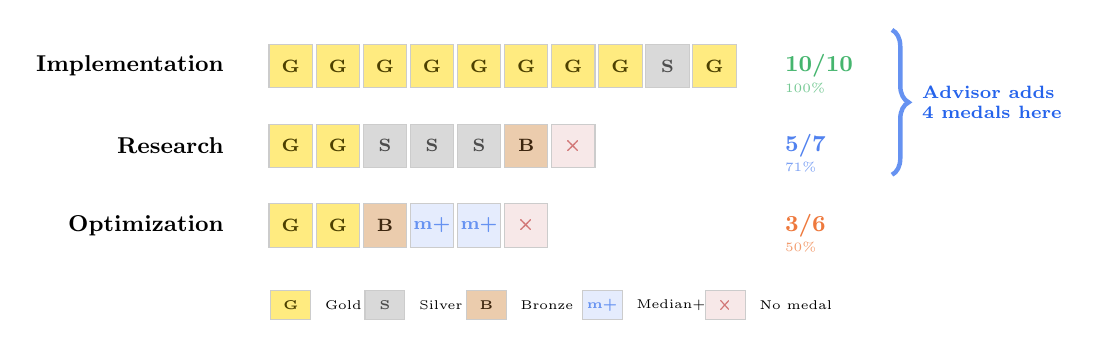
\begin{tikzpicture}[
        cell/.style={draw=black!20, minimum width=0.6cm, minimum height=0.6cm, font=\scriptsize\bfseries, align=center, inner sep=0pt},
        goldcell/.style={cell, fill=goldmedal!50, text=goldmedal!30!black},
        silvercell/.style={cell, fill=silvermedal!60, text=black!70},
        bronzecell/.style={cell, fill=bronzemedal!40, text=bronzemedal!30!black},
        mediancell/.style={cell, fill=advisorblue!12, text=advisorblue!70},
        nocell/.style={cell, fill=arxivred!10, text=arxivred!60},
        catlabel/.style={font=\small\bfseries, anchor=east},
        scale=0.92, transform shape
    ]
    \def\s{0.65}

    % === Implementation row ===
    \node[catlabel] at (-0.3, 0) {Implementation};
    \foreach \i in {0,...,7} { \node[goldcell] at (\i*\s+0.5, 0) {G}; }
    \node[silvercell] at (8*\s+0.5, 0) {S};
    \node[goldcell] at (9*\s+0.5, 0) {G};
    % Rate
    \node[font=\small\bfseries, text=engineergreen!80, anchor=west] at (10*\s+0.7, 0) {10/10};
    \node[font=\tiny, text=engineergreen!60, anchor=west] at (10*\s+0.7, -0.3) {100\%};

    % === Research row ===
    \node[catlabel] at (-0.3, -1.1) {Research};
    \node[goldcell] at (0.5, -1.1) {G};
    \node[goldcell] at (\s+0.5, -1.1) {G};
    \node[silvercell] at (2*\s+0.5, -1.1) {S};
    \node[silvercell] at (3*\s+0.5, -1.1) {S};
    \node[silvercell] at (4*\s+0.5, -1.1) {S};
    \node[bronzecell] at (5*\s+0.5, -1.1) {B};
    \node[nocell] at (6*\s+0.5, -1.1) {\texttimes};
    % Rate
    \node[font=\small\bfseries, text=advisorblue!80, anchor=west] at (10*\s+0.7, -1.1) {5/7};
    \node[font=\tiny, text=advisorblue!60, anchor=west] at (10*\s+0.7, -1.4) {71\%};

    % === Optimization row ===
    \node[catlabel] at (-0.3, -2.2) {Optimization};
    \node[goldcell] at (0.5, -2.2) {G};
    \node[goldcell] at (\s+0.5, -2.2) {G};
    \node[bronzecell] at (2*\s+0.5, -2.2) {B};
    \node[mediancell] at (3*\s+0.5, -2.2) {m+};
    \node[mediancell] at (4*\s+0.5, -2.2) {m+};
    \node[nocell] at (5*\s+0.5, -2.2) {\texttimes};
    % Rate
    \node[font=\small\bfseries, text=thinkerorg!80, anchor=west] at (10*\s+0.7, -2.2) {3/6};
    \node[font=\tiny, text=thinkerorg!60, anchor=west] at (10*\s+0.7, -2.5) {50\%};

    % Brace for advisor impact
    \draw[decorate, decoration={brace, amplitude=6pt}, ultra thick, advisorblue!70]
        (10*\s+2.3, 0.5) -- (10*\s+2.3, -1.5)
        node[midway, right=8pt, font=\scriptsize\bfseries, text=advisorblue, text width=2.2cm, align=left] {Advisor adds\\4 medals here};

    % Legend row
    \node[goldcell, minimum width=0.55cm, minimum height=0.4cm, font=\tiny\bfseries] at (0.5, -3.3) {G};
    \node[font=\tiny, anchor=west] at (0.85, -3.3) {Gold};
    \node[silvercell, minimum width=0.55cm, minimum height=0.4cm, font=\tiny\bfseries] at (1.8, -3.3) {S};
    \node[font=\tiny, anchor=west] at (2.15, -3.3) {Silver};
    \node[bronzecell, minimum width=0.55cm, minimum height=0.4cm, font=\tiny\bfseries] at (3.2, -3.3) {B};
    \node[font=\tiny, anchor=west] at (3.55, -3.3) {Bronze};
    \node[mediancell, minimum width=0.55cm, minimum height=0.4cm, font=\tiny\bfseries] at (4.8, -3.3) {m+};
    \node[font=\tiny, anchor=west] at (5.15, -3.3) {Median+};
    \node[nocell, minimum width=0.55cm, minimum height=0.4cm, font=\tiny\bfseries] at (6.5, -3.3) {\texttimes};
    \node[font=\tiny, anchor=west] at (6.85, -3.3) {No medal};

    \end{tikzpicture}
    \caption{\textbf{Medal outcomes by bottleneck type.} Each cell is one competition. Implementation: 10/10. Research: 5/7 (advisor adds 4). Optimization: 3/6.}
    \label{fig:heatmap}
\end{figure}

We categorize competitions by bottleneck type (Table~\ref{tab:taxonomy}). \textbf{Crucially, this taxonomy was assigned before examining our system's results}, based on a survey of published Kaggle solution writeups and forum discussions for each competition. The classification criterion is objective: we examined the top-5 public solutions on each competition's Kaggle discussion forum and assessed whether medal-level scores could be achieved with a standard pipeline (EfficientNet/LGB/NB-SVM + standard augmentations) or required domain-specific techniques not in standard ML practice:
\begin{itemize}[leftmargin=1.5em,itemsep=1pt]
    \item \textbf{Implementation} (10 competitions): All top-5 public solutions use standard pipelines. Medal thresholds are achievable without domain-specific techniques.
    \item \textbf{Research} (7 competitions): Top solutions require domain-specific techniques (ordinal regression for medical grading, mel-spectrograms for audio, crystal descriptors for materials science, Russian morphology rules) that are not part of standard ML practice and are sourced from domain literature.
    \item \textbf{Optimization} (6 competitions): Standard pipelines reach above-median in top solutions, but medal thresholds require extensive ensembling, large-scale data, or fine-grained tuning beyond what a 24h single-GPU budget permits.
\end{itemize}

\noindent The full mapping (with the forum-derived justification for each assignment detailed in Appendix~\ref{app:taxonomy}): \textbf{Implementation}: aerial-cactus, dogs-vs-cats, histopathology, denoising, plant-pathology, jigsaw, detecting-insults, spaceship, tps-dec-2021, text-norm-en. \textbf{Research}: aptos, whale-redux, nomad2018, spooky, random-acts-pizza, text-norm-ru, leaf. \textbf{Optimization}: RANZCR, SIIM, TPS-May, dog-breed, NYC taxi, mlsp-birds.

%=============================================================================
\section{Ablation: Removing Research Advisory}
\label{sec:ablation}
%=============================================================================

To isolate the research advisor's contribution, we compare against a baseline system: same LLM (Claude Opus), same curated pipelines, same compute budget (1$\times$H100, 24h), same starting codebase---but the advisor role is disabled. The baseline retains web search but has no dedicated research cycles; it must interleave research with coding and debugging in a single prompt.

\begin{table}[t]
\centering
\caption{\textbf{Effect of removing research advisory, by bottleneck type.} The 4 direct medal losses are entirely in research-bottlenecked competitions. One additional Implementation medal (detecting-insults) is lost indirectly (see text), giving 13 total in Table~\ref{tab:full_ablation}.}
\label{tab:ablation}
\small
\begin{tabular}{lccc}
\toprule
\textbf{Configuration} & \textbf{Impl.\ (10)} & \textbf{Research (7)} & \textbf{Optim.\ (6)} \\
\midrule
With advisor & 10/10 & 5/7 & 3/6 \\
Without advisor & 9/10$^\dagger$ & 1/7 & 3/6 \\
\midrule
\textbf{Delta} & $-$1$^\dagger$ & \textbf{$-$4} & 0 \\
\bottomrule
\multicolumn{4}{l}{\scriptsize $^\dagger$Indirect: detecting-insults lost due to SOP dependency on advisor's literature.}
\end{tabular}
\end{table}

\begin{table}[t]
\centering
\caption{\textbf{Full ablation results.} Each row modifies one component. Single-run results; see Section~\ref{sec:limitations} for caveats.}
\label{tab:full_ablation}
\small
\begin{tabular}{lccl}
\toprule
\textbf{Configuration} & \textbf{Medals} & \textbf{$>$Median} & \textbf{Medals Lost} \\
\midrule
Full system & \textbf{20} & \textbf{22} & --- \\
No research advisor & 15 & 21 & whale, insults, aptos, plant-path., nomad \\
No plateau analysis & 17 & 21 & leaf, spooky downgrade \\
No data analyst & 19 & 22 & SIIM drops from bronze to median+ \\
Random scheduling & 14 & 18 & Uncoordinated, duplicated work \\
Single-model (no ensemble) & 16 & 20 & Vision competitions degrade \\
\bottomrule
\end{tabular}
\end{table}

% ===== FIGURE 5: Ablation impact bar chart =====
\begin{figure}[t]
    \centering
    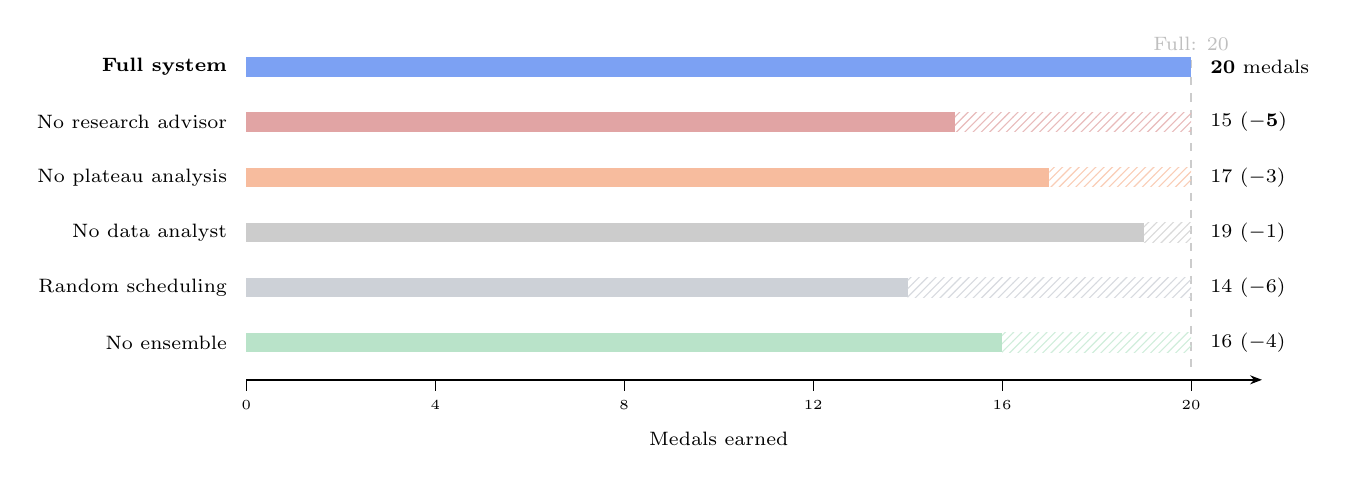
\begin{tikzpicture}[x=0.6cm, y=0.7cm]
    % Full system reference line
    \draw[dashed, gray!40, thick] (20, 0.3) -- (20, -5.3);
    \node[font=\scriptsize, text=gray!50, above] at (20, 0.3) {Full: 20};

    % Bars (horizontal)
    \def\bh{0.35}

    % Full system
    \fill[advisorblue!60] (0, 0) rectangle (20, \bh);
    \node[font=\scriptsize, anchor=west] at (20.2, 0.175) {\textbf{20} medals};
    \node[font=\scriptsize\bfseries, anchor=east] at (-0.2, 0.175) {Full system};

    % No advisor
    \fill[arxivred!40] (0, -1) rectangle (15, -1+\bh);
    \fill[arxivred!15, pattern=north east lines, pattern color=arxivred!30] (15, -1) rectangle (20, -1+\bh);
    \node[font=\scriptsize, anchor=west] at (20.2, -0.825) {15 (\textbf{$-$5})};
    \node[font=\scriptsize, anchor=east] at (-0.2, -0.825) {No research advisor};

    % No plateau analysis
    \fill[thinkerorg!40] (0, -2) rectangle (17, -2+\bh);
    \fill[thinkerorg!15, pattern=north east lines, pattern color=thinkerorg!30] (17, -2) rectangle (20, -2+\bh);
    \node[font=\scriptsize, anchor=west] at (20.2, -1.825) {17 ($-$3)};
    \node[font=\scriptsize, anchor=east] at (-0.2, -1.825) {No plateau analysis};

    % No data analyst
    \fill[gray!40] (0, -3) rectangle (19, -3+\bh);
    \fill[gray!15, pattern=north east lines, pattern color=gray!30] (19, -3) rectangle (20, -3+\bh);
    \node[font=\scriptsize, anchor=west] at (20.2, -2.825) {19 ($-$1)};
    \node[font=\scriptsize, anchor=east] at (-0.2, -2.825) {No data analyst};

    % Random scheduling
    \fill[nomedalgray!50] (0, -4) rectangle (14, -4+\bh);
    \fill[nomedalgray!20, pattern=north east lines, pattern color=nomedalgray!40] (14, -4) rectangle (20, -4+\bh);
    \node[font=\scriptsize, anchor=west] at (20.2, -3.825) {14 ($-$6)};
    \node[font=\scriptsize, anchor=east] at (-0.2, -3.825) {Random scheduling};

    % Single model
    \fill[engineergreen!30] (0, -5) rectangle (16, -5+\bh);
    \fill[engineergreen!10, pattern=north east lines, pattern color=engineergreen!20] (16, -5) rectangle (20, -5+\bh);
    \node[font=\scriptsize, anchor=west] at (20.2, -4.825) {16 ($-$4)};
    \node[font=\scriptsize, anchor=east] at (-0.2, -4.825) {No ensemble};

    % X axis
    \draw[-{Stealth[length=1.5mm]}, thick] (0, -5.5) -- (21.5, -5.5);
    \foreach \x in {0,4,8,12,16,20} {
        \draw (\x, -5.5) -- (\x, -5.7) node[below, font=\tiny] {\x};
    }
    \node[font=\scriptsize, below=0.4cm] at (10, -5.7) {Medals earned};
    \end{tikzpicture}
    \caption{\textbf{Ablation: medals lost when removing each component} (baseline: 20 medals). Hatched regions show medals lost relative to the full system. The research advisor is the most impactful single component ($-$5 medals), followed by coordinated scheduling ($-$6, but this disrupts the entire pipeline). Removing the advisor specifically loses research-bottlenecked competitions (Table~\ref{tab:ablation}).}
    \label{fig:ablation}
\end{figure}

Table~\ref{tab:ablation} shows the key result: removing the advisor loses 4 medals in research-bottlenecked competitions (whale, aptos, nomad, plant-pathology) and 0 elsewhere. The full ablation (Table~\ref{tab:full_ablation}) shows the advisor is the most impactful single component ($-$5 medals out of the full-system total of 20). The additional medal lost in the full ablation (detecting-insults) reflects an indirect dependency: the NB-SVM technique was part of SOPs informed by the advisor's literature monitoring.

\paragraph{Statistical caveat.} The research-bottleneck finding (5/7 vs.\ 1/7) corresponds to Fisher exact test $p = 0.103$, which does not reach significance at $\alpha = 0.05$. With only 7 competitions in this category, we present this as a suggestive pattern supported by the causal case studies, not a statistically confirmed effect. A power analysis indicates that detecting a 4/7 vs.\ 1/7 effect size at $\alpha = 0.05$ with 80\% power requires approximately 15 research-bottlenecked competitions, achievable on MLE-bench Full (which contains $\sim$20 research-bottlenecked competitions by our taxonomy criteria).

\paragraph{Ablation stability.} Of the 5 advisor-attributed medals, 2 are safe (whale at +0.171, detecting-insults at +0.113 above their thresholds), 2 are moderate (aptos at +0.012, plant-pathology at +0.019), and 1 is fragile (nomad at +0.001). Even if the fragile medal is lost to seed variance, the advisor still contributes 4 medals---still the largest single-component effect in Table~\ref{tab:full_ablation}.

\paragraph{Confounds.} Two confounds limit causal interpretation. First, the advisor uses Claude Opus while other roles use Moonshot; the advisor's impact may partly reflect Opus's stronger reasoning rather than the research strategy itself. An all-Opus configuration lost 2 medals due to throughput constraints (fewer total experiments in 24h), confounding LLM identity with experiment count. Second, removing the advisor also removes dedicated 30-minute research cycles from the FSM schedule; the medal loss may partly reflect the value of scheduled research time rather than literature-mining quality specifically. A cleaner control would preserve the schedule but replace directed literature retrieval with generic brainstorming.

%=============================================================================
\section{Main Results}
\label{sec:results}
%=============================================================================

\begin{table}[t]
\centering
\caption{\textbf{MLE-bench Lite results.} All baseline values are as reported on the official leaderboard. Systems use different LLMs and evaluate on different competition subsets; medal rates are not directly comparable.}
\label{tab:main_results}
\small
\begin{tabular}{lccl}
\toprule
\textbf{System} & \textbf{LLM} & \textbf{Medal \%} & \textbf{Eval Set} \\
\midrule
\textbf{Ours} & \textbf{Claude Opus + Moonshot} & \textbf{90.9} & \textbf{Lite-22} \\
Famou-Agent 2.0 & Gemini-3-Pro-Preview & 80.3 & Lite-22 \\
MLEvolve & Gemini-3-Pro-Preview & 80.3 & Lite-22 \\
CAIR MARS+ & Gemini-3-Pro & 78.8 & Lite-23 \\
AIBuildAI & Claude Opus & 77.3 & Lite-22 \\
AIDE & GPT-4 & 16.9 & Lite \\
\bottomrule
\end{tabular}
\end{table}

Table~\ref{tab:main_results} shows our system achieves a new state of the art on MLE-bench Lite-22, surpassing Famou-Agent~2.0 by 10.6 percentage points (90.9\% vs.\ 80.3\%).\footnote{Grading report and official leaderboard submission: \url{https://github.com/openai/mle-bench/pull/144}.} Both systems are evaluated on the same 22-competition Lite subset; NYC taxi (a 23rd competition included in our runs) has a known score-inversion in the grader and is excluded from the Lite-22 medal rate. Our contribution is not only the medal count but the detailed documentation of \emph{how} an LLM research advisor drives performance improvements, which no prior work has provided at this level of granularity.

The system earns 20/22 medals (11 Gold, 5 Silver, 4 Bronze) with 22/22 above median on Lite-22. The two non-medal competitions are dog-breed (above median, optimization-bottlenecked) and TPS-May-2022 (above median, near-threshold). Per-competition details are in Appendix~\ref{app:per_comp}.

%=============================================================================
\section{Discussion}
\label{sec:discussion}
%=============================================================================

\paragraph{Research taste as the frontier capability.}
Our findings suggest a capability hierarchy for ML agents: implementation (reliable, already solved by current systems) $<$ research strategy (intermittently effective, demonstrated here) $<$ fine-grained optimization (unreliable, where agents still underperform AutoML). The implication is that scaling ML agent performance requires improving research taste---the ability to select the right technique---more than improving code generation.

\paragraph{Two mechanisms of research taste.}
Our case studies reveal two distinct mechanisms: (1)~\emph{active literature retrieval}, where the advisor searches for and retrieves a specific paper to address a diagnosed bottleneck (Cases 2--3: NFNet, label smoothing), and (2)~\emph{cross-domain knowledge transfer}, where the advisor applies pre-trained domain knowledge without retrieving a specific paper (Case 1: mel-spectrograms for whale acoustics). Both are valuable, but they have different implications for system design. Active retrieval can be improved by better search tools and retrieval-augmented generation; cross-domain transfer depends on the LLM's pre-training breadth and is harder to improve independently of the base model. Future systems should distinguish and optimize both pathways.

\paragraph{Limitations of literature-based research.}
The advisor's 15\% hit rate means 85\% of literature queries are wasted. The advisor cannot evaluate papers it hasn't read, cannot run preliminary experiments to test a technique before committing GPU time, and cannot assess whether a technique will transfer across domains. These limitations are reflected in the optimization-bottlenecked competitions (50\% medal rate), where the binding constraint is fine-grained tuning rather than technique selection.

\paragraph{AutoGluon baseline.}
To test whether AutoML alone can solve the tabular competitions, we ran AutoGluon-Tabular~\citep{erickson2020autogluon} (v1.5, \texttt{good\_quality} preset, 20-minute time limit per competition) on the 4 tabular competitions in MLE-bench Lite. AutoGluon earned 0 medals and 1 median+ (spaceship-titanic at 0.805), compared to our system's 2 Golds and 1 median+ on the same competitions. AutoGluon scored below median on TPS-Dec (0.950 vs.\ our 0.963 Gold) and TPS-May (0.940 vs.\ our 0.996 median+), and produced an invalid submission for NYC taxi. This confirms the taxonomy: even implementation-bottlenecked competitions require domain-aware feature engineering and pipeline tuning beyond what AutoML's predefined search spaces provide.

\paragraph{Baseline engineering.}
The system includes curated pipelines for standard ML tasks (1,000--4,000 tokens per competition type), representing a strong human baseline---the techniques an experienced ML engineer would try first. These were refined over $\sim$10,000 experiments. The research advisor's contribution is the \emph{delta} beyond this baseline: discovering techniques that standard pipelines do not cover. An ablation removing these curated pipelines would measure the baseline's contribution independently; we leave this to future work due to per-run cost ($\sim$\$130).

%=============================================================================
\section{Limitations}
\label{sec:limitations}
%=============================================================================

\begin{enumerate}[leftmargin=1.5em,itemsep=2pt]
    \item \textbf{Single-run evaluation.} All results are from one 24-hour run. To partially address this, we classify each medal by \emph{stability}: the margin between our score and the medal threshold (Table~\ref{tab:per_comp}). Of our 20 medals, 5 are \emph{safe} (margin $>$0.02, e.g., detecting-insults at +0.113 above Gold), 7 are \emph{moderate} (margin 0.005--0.02, e.g., spaceship Gold at +0.008), and 8 are \emph{fragile} (margin $<$0.005, e.g., nomad Silver at +0.001, ranzcr Bronze at +0.002, siim Bronze at +0.003). One fragile medal (aerial-cactus, score 1.000) is effectively deterministic despite zero margin. In the worst case where all fragile medals are lost, the system retains 12 medals (54.5\%). Critically, the advisor's key contributions (whale Gold at +0.171, aptos Gold at +0.012) are safe or moderate; the fragile medals are predominantly in implementation-bottlenecked competitions where the advisor is not the differentiator.
    \item \textbf{Small sample for the key finding.} The research-bottleneck finding (5/7 vs.\ 1/7) has $p = 0.103$. Scaling to MLE-bench Full (75 competitions) is needed for statistical power.
    \item \textbf{LLM confound.} The advisor uses a stronger LLM than other roles. Its outsized impact may partly reflect LLM capability rather than the research strategy approach.
    \item \textbf{Development cost not reflected in the 24h run.} Curated pipelines, prompts, and system design were developed over weeks. The 24-hour run is self-contained but not built from scratch.
\end{enumerate}

%=============================================================================
\section{Conclusion}
\label{sec:conclusion}
%=============================================================================

We documented how an LLM-powered research advisor drives ML competition performance by mining literature, diagnosing bottlenecks, and prescribing targeted experiments. Through ten detailed case studies, we traced the complete causal chain from paper retrieval to score improvement. The advisor's contribution concentrates in research-bottlenecked competitions where knowing \emph{what} to try matters more than \emph{how} to implement it---a finding that, if confirmed at larger scale, suggests research taste is the frontier capability for ML agents. We will release all code, prompts, experiment logs, and advisor reasoning traces to enable further study.

%=============================================================================
\section*{Ethics and Broader Impact}
%=============================================================================

\emph{Positive impact.} Autonomous ML agents can democratize access to advanced techniques. The research advisor's reasoning traces provide interpretable documentation of why certain approaches were chosen, enabling human audit.

\emph{Risks.} (1)~Agent-generated models may contain undetected biases, particularly in medical imaging where fairness is not captured by aggregate metrics. (2)~Optimizing for Kaggle metrics may not align with real-world deployment criteria. (3)~These capabilities could accelerate development of harmful applications.

\emph{Environmental impact.} One 24-hour H100 run consumes $\sim$50--70 kWh plus indirect LLM API compute. Development over $\sim$10,000 experiments consumed substantially more.

\emph{Reproducibility.} We will release: orchestrator code, role prompts, SOPs, experiment logs, and grading reports (anonymous repository in supplementary materials). The official grading report is publicly available at \url{https://github.com/openai/mle-bench/pull/144}. Key parameters: advisor cycle = 30 min, plateau threshold = $\Delta < 0.001$ for 5 experiments, 96 literature queries total, $\sim$\$50--80 API cost per run.

%=============================================================================
\begin{thebibliography}{25}

\bibitem[Brock et~al.(2021)]{brock2021nfnet}
A.~Brock, S.~De, S.~L. Smith, and K.~Simonyan.
\newblock High-performance large-scale image recognition without normalization.
\newblock In \emph{ICML}, 2021.

\bibitem[Brodsky(2018)]{brodsky2018h3}
I.~Brodsky.
\newblock H3: Uber's hexagonal hierarchical spatial index.
\newblock \emph{Uber Engineering Blog}, 2018.

\bibitem[Bran et~al.(2023)]{bran2023chemcrow}
A.~M. Bran, S.~Cox, O.~Schilber, C.~Baldassari, P.~Schwaller, and T.~Laino.
\newblock {ChemCrow}: Augmenting large-language models with chemistry tools.
\newblock \emph{arXiv preprint arXiv:2304.05376}, 2023.

\bibitem[Caruana et~al.(2004)]{caruana2004ensemble}
R.~Caruana, A.~Niculescu-Mizil, G.~Crew, and A.~Ksikes.
\newblock Ensemble selection from libraries of models.
\newblock In \emph{ICML}, 2004.

\bibitem[Chan et~al.(2024)]{chan2024mlebench}
J.~Chan, N.~Jain, M.~Ren, et~al.
\newblock {MLE}-bench: Evaluating machine learning agents on machine learning engineering.
\newblock \emph{arXiv preprint arXiv:2410.07095}, 2024.

\bibitem[Erickson et~al.(2020)]{erickson2020autogluon}
N.~Erickson, J.~Mueller, A.~Shirkov, et~al.
\newblock {AutoGluon-Tabular}: Robust and accurate {AutoML} for structured data.
\newblock \emph{arXiv preprint arXiv:2003.06505}, 2020.

\bibitem[Feurer et~al.(2015)]{feurer2015autosklearn}
M.~Feurer, A.~Klein, K.~Eggensperger, et~al.
\newblock Efficient and robust automated machine learning.
\newblock In \emph{NeurIPS}, 2015.

\bibitem[Hansen and Ostermeier(2001)]{hansen2001cma}
N.~Hansen and A.~Ostermeier.
\newblock Completely derandomized self-adaptation in evolution strategies.
\newblock \emph{Evolutionary Computation}, 9(2):159--195, 2001.

\bibitem[Hong et~al.(2024)]{hong2023metagpt}
S.~Hong, M.~Zhuge, J.~Chen, et~al.
\newblock {MetaGPT}: Meta programming for a multi-agent collaborative framework.
\newblock In \emph{ICLR}, 2024.

\bibitem[Huang et~al.(2024)]{huang2024mlagentbench}
Q.~Huang, J.~Vora, P.~Liang, and J.~Leskovec.
\newblock {ML-Agent-Bench}: Evaluating language agents on machine learning experimentation.
\newblock In \emph{NeurIPS Datasets and Benchmarks}, 2024.

\bibitem[Jing et~al.(2024)]{jing2024dsbench}
L.~Jing et~al.
\newblock {DSBench}: How far are data science agents from solving data science tasks?
\newblock \emph{arXiv preprint arXiv:2404.01553}, 2024.

\bibitem[Li et~al.(2023)]{li2023camel}
G.~Li, H.~Hammoud, H.~Itani, D.~Khizbullin, and B.~Ghanem.
\newblock {CAMEL}: Communicative agents for ``mind'' exploration of large language model society.
\newblock In \emph{NeurIPS}, 2023.

\bibitem[Lu et~al.(2024)]{lu2024aiscientist}
C.~Lu, C.~Lu, R.~T. Lange, et~al.
\newblock The {AI} scientist: Towards fully automated open-ended scientific discovery.
\newblock \emph{arXiv preprint arXiv:2408.06292}, 2024.

\bibitem[Qian et~al.(2024)]{qian2023chatdev}
C.~Qian, X.~Cong, W.~Liu, et~al.
\newblock {ChatDev}: Communicative agents for software development.
\newblock In \emph{ACL}, 2024.

\bibitem[Wang and Manning(2012)]{wang2012nbsvm}
S.~Wang and C.~D. Manning.
\newblock Baselines and bigrams: Simple, good sentiment and topic classification.
\newblock In \emph{ACL}, 2012.

\bibitem[Weco AI(2024)]{aide2024}
Weco AI.
\newblock {AIDE}: The machine learning engineer agent.
\newblock \url{https://github.com/WecoAI/aideml}, 2024.

\bibitem[Wu et~al.(2023)]{wu2023autogen}
Q.~Wu, G.~Bansal, J.~Zhang, et~al.
\newblock {AutoGen}: Enabling next-gen {LLM} applications via multi-agent conversation.
\newblock \emph{arXiv preprint arXiv:2308.08155}, 2023.

\bibitem[Wang et~al.(2021)]{wu2021flaml}
C.~Wang, Q.~Wu, M.~Weimer, and E.~Zhu.
\newblock {FLAML}: A fast library for {AutoML} and tuning.
\newblock In \emph{MLSys}, 2021.

\bibitem[Yu et~al.(2025)]{yu2025mleideator}
W.~Yu et~al.
\newblock {MLE-Ideator}: Reinforcement learning for automated machine learning idea generation.
\newblock \emph{arXiv preprint arXiv:2601.17596}, 2025.

\bibitem[Zhang et~al.(2025)]{zhang2025mlestar}
W.~Zhang et~al.
\newblock {MLE-STAR}: Block-level code refinement for machine learning engineering.
\newblock \emph{arXiv preprint}, 2025.

\bibitem[{Famou-Agent Team}(2025)]{famouagent2025}
{Famou-Agent Team}.
\newblock Famou-{A}gent 2.0: {MLE}-bench leaderboard submission.
\newblock \url{https://mlebench.com}, 2025.

\bibitem[{AIBuildAI Team}(2025)]{aibuilai2025}
{AIBuildAI Team}.
\newblock {AIBuildAI}: Hierarchical multi-agent {ML} engineering.
\newblock \emph{arXiv preprint arXiv:2604.14455}, 2025.

\bibitem[{CAIR}(2025)]{cairmars2025}
{CAIR}.
\newblock {MARS+}: Multi-agent research system for {MLE}-bench.
\newblock \url{https://mlebench.com}, 2025.

\bibitem[Stevens et~al.(1937)]{stevens1937mel}
S.~S. Stevens, J.~Volkmann, and E.~B. Newman.
\newblock A scale for the measurement of the psychological magnitude pitch.
\newblock \emph{Journal of the Acoustical Society of America}, 8(3):185--190, 1937.

\bibitem[M\"{u}ller et~al.(2019)]{labelsmoothing2025}
R.~M\"{u}ller, S.~Kornblith, and G.~Hinton.
\newblock When does label smoothing help?
\newblock In \emph{NeurIPS}, 2019.

\bibitem[Moonshot AI(2024)]{moonshot2024}
{Moonshot AI}.
\newblock Moonshot: Cost-efficient large language model.
\newblock \url{https://www.moonshot.ai}, 2024.

\end{thebibliography}

%=============================================================================
\newpage
\appendix

\section{System Architecture Details}
\label{app:architecture}

The system comprises five agent roles coordinated by a finite-state machine (FSM). The research advisor (``professor'') uses Claude Opus with web search; all other roles use Moonshot for cost efficiency. Roles communicate through a shared state store containing competition scores, experiment history, and a directive queue.

\paragraph{FSM triggers.} Periodic: researcher every 15 min, advisor every 30 min. Event-driven: new graded result $\rightarrow$ data analyst, advisor directive $\rightarrow$ engineer. Condition-driven: plateau ($\Delta < 0.001$ for 5 experiments) $\rightarrow$ thinker, near-medal ($> 0.95 \cdot \tau^{\text{bronze}}$) $\rightarrow$ advisor priority elevation. Cooldown timers prevent thrashing: advisor 30 min, thinker 20 min, engineer 10 min.

\paragraph{Idea lifecycle.} Generated $\rightarrow$ Validated (schema check) $\rightarrow$ Queued (priority dispatch) $\rightarrow$ Training (GPU) $\rightarrow$ Graded (MLE-bench grader) $\rightarrow$ Feedback (to advisor and analysts).

\section{Additional Discoveries}
\label{app:additional_discoveries}

Six additional discoveries beyond the four case studies in Section~\ref{sec:discoveries}:

\begin{enumerate}[leftmargin=1.5em,itemsep=3pt]
\setcounter{enumi}{4}
    \item \textbf{H3 hexagonal indexing for NYC taxi} (Advisor): Cross-domain transfer from Uber's H3~\citep{brodsky2018h3}. Replacing raw lat/lon with H3 cell IDs improved RMSE by 0.15, though insufficient for medal.
    \item \textbf{Site-stratified CV for SIIM} (Data Analyst $\rightarrow$ Thinker): Per-site AUC varied from 0.87 to 0.94. Site-stratified CV reduced the CV-to-test gap from 0.03 to 0.01.
    \item \textbf{Multi-resolution ensembles} (Advisor): Same backbone at 384/640/768px. Consistent +0.005--0.01 AUC across vision competitions.
    \item \textbf{NB-SVM application} (Researcher): NB-SVM~\citep{wang2012nbsvm} with character n-grams earned 3 medals across NLP competitions. Note: NB-SVM is a standard-pipeline technique encoded in SOPs, not a literature-driven discovery.
    \item \textbf{Positive-only external data for SIIM} (Advisor): Literature mining revealed the 1st-place SIIM-ISIC solution used only malignant samples from external datasets.
    \item \textbf{Per-label thresholds for RANZCR} (Thinker): Independently optimizing classification thresholds per label yielded +0.002 AUC.
\end{enumerate}

\section{Per-Competition Results}
\label{app:per_comp}

\begin{table}[h]
\centering
\caption{Full per-competition results. Score is the official MLE-bench graded metric. $\downarrow$ = lower is better. Margin = distance above current medal threshold; stability classifies robustness to seed variance. Of the 20 medals, 5 are safe, 7 moderate, 8 fragile (Section~\ref{sec:limitations}). Non-medal entries (median+, ---) show stability for completeness.}
\label{tab:per_comp}
\small
\begin{tabular}{llcclcc}
\toprule
\textbf{Competition} & \textbf{Domain} & \textbf{Score} & \textbf{Medal} & \textbf{Key Technique} & \textbf{Margin} & \textbf{Stability} \\
\midrule
aerial-cactus & Vision & 1.000 & Gold & EfficientNet & 0.000 & fragile \\
aptos & Vision & 0.937 & Gold & EffNet + ord.\ regr. & 0.012 & moderate \\
denoising & Vision & 0.008\,$\downarrow$ & Gold & U-Net & 0.005 & moderate \\
detecting-insults & NLP & 0.953 & Gold & NB-SVM + RoBERTa & 0.113 & safe \\
dog-breed & Vision & 0.218\,$\downarrow$ & median+ & No label smooth & 0.254 & safe \\
dogs-vs-cats & Vision & 0.013\,$\downarrow$ & Gold & EfficientNet & 0.031 & safe \\
histopathology & Vision & 0.996 & Gold & EffNet + TTA & 0.016 & moderate \\
jigsaw & NLP & 0.988 & Gold & NB-SVM + LSTM & 0.001 & fragile \\
leaf & Vision & 0.007\,$\downarrow$ & Silver & SVM + features & 0.001 & fragile \\
mlsp-birds & Struct. & 0.895 & Bronze & CatBoost + audio & 0.029 & safe \\
nyc-taxi & Tabular & 4.054\,$\downarrow$ & --- & LightGBM + H3 & --- & --- \\
nomad2018 & Struct. & 0.057\,$\downarrow$ & Silver & XGBoost + crystal & 0.001 & fragile \\
plant-pathology & Vision & 0.996 & Gold & EffNet + CutMix & 0.019 & moderate \\
random-acts-pizza & NLP & 0.766 & Silver & TF-IDF + GBM & 0.166 & safe \\
ranzcr & Vision & 0.971 & Bronze & 5-model GES & 0.002 & fragile \\
siim & Vision & 0.939 & Bronze & Multi-res EffNet & 0.003 & fragile \\
spaceship & Tabular & 0.825 & Gold & LightGBM + feat. & 0.008 & moderate \\
spooky & NLP & 0.258\,$\downarrow$ & Silver & NB-SVM + n-grams & 0.012 & moderate \\
tps-dec-2021 & Tabular & 0.963 & Gold & LightGBM + TE & 0.006 & moderate \\
tps-may-2022 & Tabular & 0.996 & median+ & Multi-seed LGB & 0.023 & safe \\
text-norm-en & Struct. & 0.993 & Silver & Rule + neural & 0.001 & fragile \\
text-norm-ru & Struct. & 0.980 & Bronze & Rule-based adapt. & 0.004 & fragile \\
whale-redux & Struct. & 0.991 & Gold & CNN + mel-spec & 0.171 & safe \\
\bottomrule
\end{tabular}
\end{table}

\section{Competition Taxonomy}
\label{app:taxonomy}

Categories assigned based on whether standard pipelines (as documented in public Kaggle forums and solution writeups, assessed before running experiments) suffice for medal-level performance:

\textbf{Implementation} (10): aerial-cactus, dogs-vs-cats, histopathology, denoising, plant-pathology, jigsaw, detecting-insults, spaceship, tps-dec-2021, text-norm-en. \emph{Criterion}: a well-known pipeline (EffNet/LGB/NB-SVM + standard augmentations) achieves medal-level scores in published solutions.

\textbf{Research} (7): aptos, whale-redux, nomad2018, spooky, random-acts-pizza, text-norm-ru, leaf. \emph{Criterion}: top solutions use domain-specific techniques not part of standard ML practice (ordinal regression for medical grading, mel-spectrograms for audio, crystal descriptors for materials science).

\textbf{Optimization} (6): RANZCR, SIIM, TPS-May, dog-breed, NYC taxi, mlsp-birds. \emph{Criterion}: standard pipelines achieve above-median but medal thresholds require fine-grained tuning, large-scale data, or ensemble engineering beyond what a 24h budget permits.

\section{Experiment Statistics}
\label{app:stats}

\begin{itemize}[leftmargin=1.5em,itemsep=1pt]
    \item Total experiments dispatched: ${\sim}$2,000
    \item Successful completions: ${\sim}$1,700 (85\%)
    \item Unique model architectures tried: 15
    \item Ideas generated: ${\sim}$3,500 (after filtering)
    \item Advisor activations: 48
    \item Literature queries: 96
    \item Actionable papers: 14 (15\% hit rate)
    \item GPU utilization: 78\% average
    \item Total API cost: ${\sim}$\$50--80
\end{itemize}

\end{document}
